\section{Convolutional Neural Networks}
\subsection{Task 1: Theory}
\subsubsection*{a)}
Listing the equations for calculating the resulting height and width: 
\begin{align}
    W_{i + 1} &= (W_i - F_W + 2 P_W)/S_W + 1 \\
    H_{i + 1} &= (H_i - F_H + 2 P_H)/S_H + 1
\end{align}

Now defining: 
\begin{align*}
    S_W &= S_H = 1 \\
    F_W &= F_H = 5 \\
    H_2 &= H_1 = H \\
    W_2 &= W_1 = W
\end{align*}

Then we get for the width:
\begin{align*}
    W_2 &= (W_1 - F_W + 2 P_W)/S_W + 1 \\
    W - 1 &= W - 5 + 2 P_W \\
    2 P_W &= 4 \\
    P_W &= 2
\end{align*}

And for height: 
\begin{align*}
    H_2 &= (H_1 - F_H + 2 P_H)/S_H + 1 \\
    H - 1 &= H - 5 + 2 P_H \\
    2 P_H &= 4 \\
    P_H &= 2
\end{align*}

So we should therefore be padding with $P_H = 2$ and $P_W = 2$. 

\subsubsection*{c)}
Now defining: 
\begin{align*}
    S_H &= S_W = 1 \\
    P_H &= P_W = 0 \\
    H_1 &= W_1 = 512 \\
    H_2 &= W_2 = 504 \\
    F_H &= ? \\
    F_W &= ?
\end{align*}

Then using the same equations as above, we calculate: 
\begin{align*}
    H_2 &= (H_1 - F_H + 2 * P_H) / S_H + 1 \\
    504 &= (512 - F_H + 2 * 0) / 1 + 1 \\
    F_H &= 512 + 1 - 504 = 9 \\ \\
    W_2 &= (W_1 - F_W + 2 * P_W) / S_W + 1 \\
    504 &= (512 - F_W + 2 * 0) / 1 + 1 \\
    F_W &= 512 + 1 - 504 = 9
\end{align*}

We also knew from the task that the kernel was supposed to be square, and its dimensions odd, which we can confirm from the result. The kernel must therefore be of the size $9 x 9$. 

\subsection*{d)}
Starting with subsampling with neighbourhoods, defining: 
\begin{align*}
    H_1 &= W_1 = 512 \\
    S_H &= S_W = 2 \\
    P_H &= P_W = 0 \\
    F_H &= F_W = 2 \\
    H_2 &= ? \\
    W_2 &= ?
\end{align*}

Then we get: 
\begin{align*}
    H_2 &= (H_1 - F_H + 2 * P_H) / S_H + 1 \\
    &= (512 - 2 + 2 * 0) / 2 + 1 = 255 \\
    W_2 &= (W_1 - F_W + 2 * P_W) / S_W + 1 \\
    &= (512 - 2 + 2 * 0) / 2 + 1 = 255
\end{align*}

Then, using the same information utilized above, we define: 
\begin{align*}
    H_1 &= W_1 = 255 \\
    S_H &= S_W = 1 \\
    P_H &= P_W = 0 \\
    F_H &= F_W = 9 \\
    H_2 &= ? \\
    W_2 &= ?
\end{align*}

Then we calculate: 
\begin{align*}
    H_2 &= (H_1 - F_H + 2 * P_H) / S_H + 1 \\
    &= (255 - 9 + 2 * 0) / 1 + 1 = 247 \\
    W_2 &= (W_1 - F_W + 2 * P_W) / S_W + 1 \\
    &= (255 - 9 + 2 * 0) / 1 + 1 = 247
\end{align*}

Then the spatial dimensions of the pooled feature maps in the first layer would be $247x247$. 

\subsection*{e)}
Uncertain about this question. Wouldn't it just be the same as the number of feature maps? In that case, 12... 

\subsection*{f)}
Defining: 
\begin{align*}
    H_1 &= W_1 = 247 \\
    S_H &= S_W = 1 \\
    P_H &= P_W = 0 \\
    F_H &= F_W = 3 \\
    H_2 &= ? \\
    W_2 &= ?
\end{align*}

Then: 
\begin{align*}
    H_2 &= (H_1 - F_H + 2 * P_H) / S_H + 1 \\
    &= (247 - 3 + 2 * 0) / 1 + 1 = 245 \\
    W_2 &= (W_1 - F_W + 2 * P_W) / S_W + 1 \\
    &= (247 - 3 + 2 * 0) / 1 + 1 = 245
\end{align*}

Therefore, the sizes of the feature map of the second layer would be $245 x 245$. 

\subsection*{g)}
Defining the $0$-layer as the input layer, so that the other layers can be defined incrementally as well as being the given layer in the table. Furthermore, superscript will be used to specify the layer type. I will use $C$ for Conv2D, $M$ for MaxPool2D

\begin{align*}
    H_0 &= W_0 = 32 \\
    C_0 &= 3 \\
    S_H^C &= S_W^C = 1 \\
    P_H^C &= P_W^C = 2 \\
    F_H^C &= F_W^C = 5 \\
    S_H^M &= S_W^M = 2 \\
    P_H^M &= P_W^M = 0 \\
    F_H^M &= F_W^M = 2 \\
    C_1 &= 32 \\ 
    C_2 &= 64 \\
    C_3 &= 128
\end{align*}

The flattening-layer will then convert the $4x4x128$ result from layer 3 to a vector of size $4 * 4 * 128 = 2048$. Then this is mapped with to 64 hidden units, and finally to the 10, representing the ten different classes (digits). 

\begin{equation}
    \label{eq:num_params_cnn}
    n_{i+1} = F_H^C * F_W^C * C_i * C_{i+1} + C_{i+1} = 25 * C_i * C_{i+1} + C_{i+1} 
\end{equation}

To calculate the number of parameters, we look at each filters individually. Using \cref{eq:num_params_cnn}, we can calculate the number of parameters for each layer: 

\begin{align*}
    n_1 &= 25 * 3  * 32  + 32 = 2432 \\
    n_2 &= 25 * 32 * 64  + 64 = 51264 \\
    n_3 &= 25 * 64 * 128 + 128 = 204928 \\
    n_4 &= 4 * 4 * 128 * 64 + 1 = 131073 \\
    n_5 &= 64 * 10 + 1 = 641 \\
    n   &= \sum_{i = 1}^5 n_i = 390338
\end{align*}

I also calculate the spatial dimensions of the layers. This wasn't strictly needed to calculate the number of parameters, but was useful for task 2: 
\begin{align*}
    H_1^C &= (H_0 - F_H^C + 2 * P_H^C) / S_H^C + 1   = (32 - 5 + 2 * 2) / 1 + 1 = 32 \\
    H_1^M &= (H_1^C - F_H^M + 2 * P_H^M) / S_H^M + 1 = (32 - 2 + 2 * 0) / 2 + 1 = 16 \\
    H_2^C &= (H_1^M - F_H^C + 2 * P_H^C) / S_H^C + 1 = (16 - 5 + 2 * 2) / 1 + 1 = 16 \\
    H_2^M &= (H_2^C - F_H^M + 2 * P_H^M) / S_H^M + 1 = (16 - 2 + 2 * 0) / 2 + 1 = 8 \\
    H_3^C &= (H_2^M - F_H^C + 2 * P_H^C) / S_H^C + 1 = (8  - 5 + 2 * 2) / 1 + 1 = 8 \\
    H_3^M &= (H_3^C - F_H^M + 2 * P_H^M) / S_H^M + 1 = (8  - 2 + 2 * 0) / 2 + 1 = 4 \\
    W_1^C &= (W_0 - F_W^C + 2 * P_W^C) / S_W^C + 1   = (32 - 5 + 2 * 2) / 1 + 1 = 32 \\
    W_1^M &= (W_1^C - F_W^M + 2 * P_W^M) / S_W^M + 1 = (32 - 2 + 2 * 0) / 2 + 1 = 16 \\
    W_2^C &= (W_1^M - F_W^C + 2 * P_W^C) / S_W^C + 1 = (16 - 5 + 2 * 2) / 1 + 1 = 16 \\
    W_2^M &= (W_2^C - F_W^M + 2 * P_W^M) / S_W^M + 1 = (16 - 2 + 2 * 0) / 2 + 1 = 8 \\
    W_3^C &= (W_2^M - F_W^C + 2 * P_W^C) / S_W^C + 1 = (8  - 5 + 2 * 2) / 1 + 1 = 8 \\
    W_3^M &= (W_3^C - F_W^M + 2 * P_W^M) / S_W^M + 1 = (8  - 2 + 2 * 0) / 2 + 1 = 4 
\end{align*}

\newpage
\subsection{Task 2: Programming}

% \begin{figure}[]
%     \centering
%     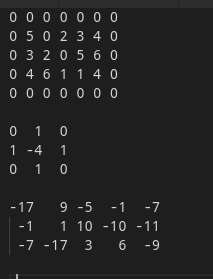
\includegraphics[width=1.00\textwidth]{figures/convolution_by_hand.png}
%     \caption{Convolution by hand}
%     \label{fig:kernel_convolution}
% \end{figure}

\subsubsection*{a)}
\begin{figure}[]
    \centering
    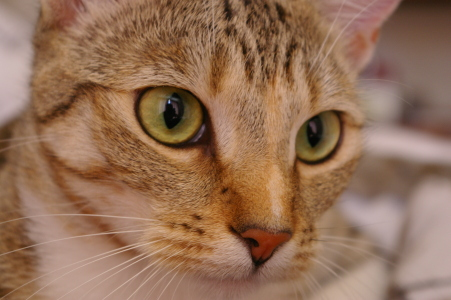
\includegraphics[width=1.00\textwidth]{figures/image_processed/chelsea.png}
    \caption{Chelsea without maxpooling}
    \label{fig:chelsea_original}
\end{figure}

\begin{figure}[]
    \centering
    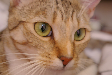
\includegraphics[width=1.00\textwidth]{figures/image_processed/chelsea_maxpooled.png}
    \caption{Chelsea with maxpooling}
    \label{fig:chelsea_maxpooled}
\end{figure}

\begin{figure}[]
    \centering
    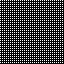
\includegraphics[width=1.00\textwidth]{figures/image_processed/checkerboard.png}
    \caption{Checkerboard without maxpooling}
    \label{fig:checkerboard_original}
\end{figure}

\begin{figure}[]
    \centering
    
\includegraphics[width=1.00\textwidth]{figures/image_processed/checkerboard_maxpooled.png}
    \caption{Checkerboard with maxpooling}
    \label{fig:checkerboard_maxpooled}
\end{figure}

\subsubsection*{b)}
% Final Validation loss: 0.06696378275700904. Final Validation accuracy: 0.9758

\subsubsection*{c)}
% Final Validation loss: 0.021018466441450896. Final Validation accuracy: 0.9932

\subsubsection*{d)}

\subsubsection*{e)}